\chapter {Introducción}
\section{Introducción al problema}

	\begin{paragraph}
			 Tradicionalmente, en el mundo IT han existido dos departamentos claramente diferenciados entre sí. Desarrolladores y Operaciones. Éstos hacen referencia a dos tipos de informático. Por un lado el desarrollador de aplicaciones, que se encarga de escribir código para cumplir unos requisitos funcionales y darle forma al producto. Este primer grupo se caracteriza por únicamente preocuparse de que la aplicación funcione correctamente en su entorno de desarrollo y que cumpla las funcionalidades descritas por el cliente. Por otro lado nos encontramos la otra cara de la moneda, el perfil de operaciones o sistemas o, como lo llaman algunos, 'sysadmin'. Éstos no se encargan de desarrollar aplicaciones, se encargan de realizar todas las operaciones que hay alrededor de una aplicación a nivel de sistemas, a la hora de lanzarla en un entorno de producción. Un sysadmin se encargará de toda la parte de testing y despliegue así como del mantenimiento de los servidores una vez desplegada la aplicación. \\
			 Alguno ya sabrá y se habrá dado cuenta de que esta diferenciación y separación de un trabajo en dos bandos diferenciados va a causar problemas a largo plazo y no se equivoca. De hecho, si preguntas a cualquiera que haya trabajado con ésta filosofía de trabajo te explicará rápidamente los problemas. Al tener los equipos separados, el desarrollador únicamente se preocupa de que su aplicación funcione en su entorno de desarrollo, lavándose las manos y dejándo toda la responsabilidad en manos del equipo de sistemas. Del mismo modo, el equipo de sistemas ante cualquier fallo en la aplicación, echarán las culpas al equipo de desarrollo, ya que es su trabajo que la aplicación funcione correctamente y así sucesivamente... Son habituales los comentarios del tipo: 'Si a mi en local me funciona...' o ante cualquier fallo en producción: 'La aplicación funciona correctamente, seguro que son los sistemas...'. Como era de suponer, este enfoque no iba a durar mucho tiempo ya que los inconvenientes de esta forma de trabajar (sobretodo en equipos grandes) son insostenibles. Desafortunadamente hoy en día sigue habiendo empresas con esta filosofía de trabajo, sobretodo empresas con una larga trayectoría que se niegan a cambiar algo que 'ya funciona'. Este trabajo pretende justamente facilitar la adoptación de técnicas DevOps a una pequeña empresa, cambiando el enfoque y la forma de trabajar de los departamentos de desarrollo y sistemas.
	\end{paragraph}

\section{Motivación}

	\begin{paragraph}
		Allá por 2007, en la Agile Conference de Toronto, Andrew Shafer (fundador de Puppet) da una charla sobre aplicar la metodología Agile a la infraestructura. Su único oyente Patrick Debois interesado por el tema, mantiene una larga conversación sobre el tema y deciden fundar una lista de correo Agile System Administration. Este momento ha sido crucial para la filosofía DevOps ya que es en esta lista donde empiezan a germinar algunos conceptos conocidos hoy día como integración contínua, entrega contínua, infraestructura como código, etc.\\
		Es en 2009 cuando se produce el famoso congreso  'O'reilly Velocity Conference' donde se realiza una charla llamada '10 Deploys per day'. En esta charla se empieza a plantear seriamente la fusión de los departamentos de Desarrollo y Operaciones. A raíz de esta charla nacen los llamados DevOpsdays, desarrolladores y equipo de operaciones empiezan a trabajar conjuntamente dando ideas de como poder fusionar ambos departamentos. Los DevOpsdays, rápidamente se extienden por todo el mundo popularizándose el término DevOps como fusión de Desarrollo y Operaciones.
	\end{paragraph}
\section{Conceptos básicos}
		\begin{paragraph}
			A continuación se van a describir uno a uno, los conceptos básicos para entender este proyecto. Son conceptos claves sin los cuales un lector inexperto no comprenderá ni el problema ni la solución adoptada para el problema.
		\end{paragraph}
	\subsection{DevOps}
		\begin{paragraph}
			El término DevOps es una fusión de las dos palabras Desarrollo y Operaciones. DevOps es una filosofía, una forma de abordar el desarrollo de software. El objetivo de DevOps es fusionar los departamentos Desarollo y Operaciones de forma que sea más fácil y rápida la creación de software. La siguiente imagen define el término:
			
			\begin{figure}[!hbt]
				\centering
				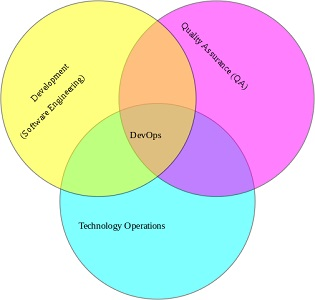
\includegraphics[scale=0.75]{imagenes/Introduccion/Conceptos_Basicos/devops.jpg}
				\caption[¿Qué es DevOps?]{¿Qué es DevOps? \cite{WhatIsDe1:online}}
				\label{termino_devops}
			\end{figure}
			 
		\end{paragraph}
	\subsection{Integración Contínua (CI)}
		\begin{paragraph}
			La Integración Contínua o CI para abreviar, es uno de los pilares de la filosofía DevOps. La integración contínua se basa en haer integraciones automáticas de un proyecto lo más a menudo posible para poder detectar fallos rápidamente. La Integración Contínua consta de dos partes: compilación y ejecución de tests de un proyecto.
			
			\begin{figure}[!hbt]
				\centering
				\includegraphics[scale=0.45]{imagenes/Introduccion/Conceptos_Basicos/ci.png}
				\caption[Integración Contínua]{Integración Contínua \cite{Alcanzan90:online} }
				\label{integracion_continua} 
			\end{figure}
		\end{paragraph}
	\subsection{Despliegue contínuo (CD)}
		\begin{paragraph}
			El Despligue Contínuo o CD por sus siglas en inglés 'Continous Delivery' complementa a la integración contínua desplegando el proyecto software en los servidores de producción una vez ha pasado el proceso de la integración contínua. Gracias a CD podemos garantizar entregas rápidas y seguras de software.
			
			\begin{figure}[!hbt]
				\centering
				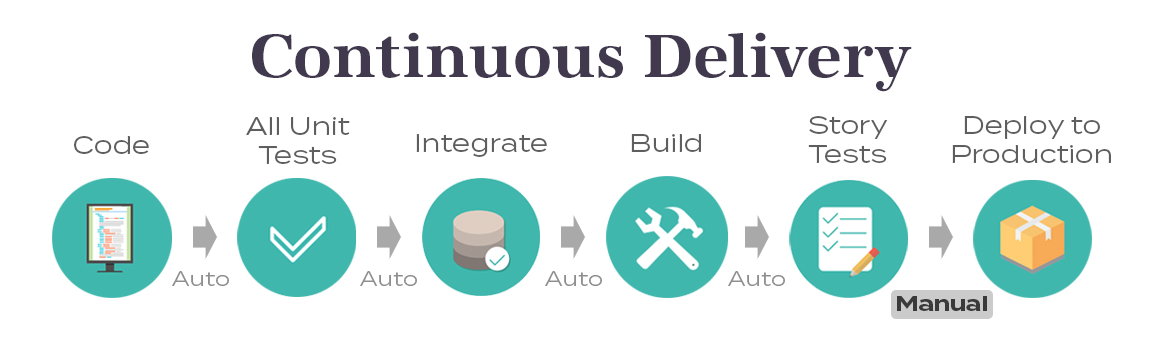
\includegraphics[scale=0.35]{imagenes/Introduccion/Conceptos_Basicos/CD.png}
				\caption[Despliegue Contínuo]{Despliegue Contínuo \cite{continuo84:online}}
				\label{despligue_continuo} 
			\end{figure}
		\end{paragraph}
	\subsection{Infraestructura como Código (IaaC)}
		\begin{paragraph}
			La infraestructura cómo código pretende tratar los servidores y toda la infraestructura alrededor de una organización como un software de programación. De este modo, la infraestructura está escrita en ficheros de configuración y es fácilmente replicable y testeable. Este concepto al igual que los dos anteriores está íntimamente ligado con el término DevOps, ya que es uno de los primeros pasos a adoptar. IaaC pretende difuminar la línea entre el código que ejecutan las aplicaciones y el código que configura la infraestructura. IaaC acerca a los desarrolladores al equipo de operaciones o administradores de sistemas. \\
			De esta manera no únicamente se testea el software antes de ser lanzado, si no también la infraestructura. A continuación se muestra como sería el cauce de trabajo siguiendo los principios de IaaC.
			
			\begin{figure}[!hbt]
				\centering
				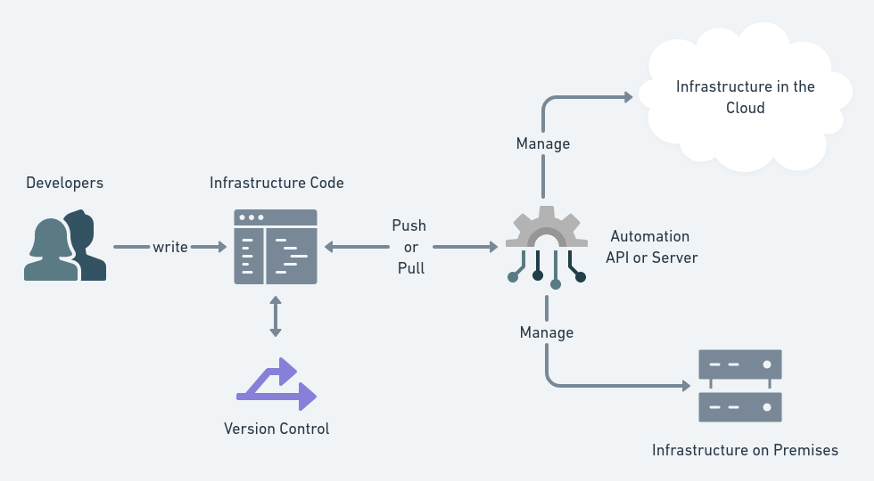
\includegraphics[scale=0.45]{imagenes/Introduccion/Conceptos_Basicos/IaaC.png}
				\caption[Infraestructura como Código]{Infraestructura como Código \cite{WhatIsIaaC:online}}
				\label{infraestructura_como_codigo} 
			\end{figure}
		\end{paragraph}
	
\section{Estado del arte}
	\begin{paragraph}
		En esta sección se va a comentar el estado actual de proyectos parecidos al que se describe en este documento. Sin embargo, antes de abordar esta cuestión me gustaría hacer un pequeño análisis de cómo ha evolucionado el mercado laboral de este tipo de puestos de trabajo para hacer énfasis en la importancia de todo lo mencionado anteriormente.
	\end{paragraph}

	\subsection{Introducción}
		\begin{paragraph}
			Es una realidad que cada día más las empresas optan por soluciones Cloud y es bastante sencillo para un programador medio crear cauces de desarrollo y despliegue para sus aplicaciones en éstos proveedores Cloud y convertirse en todo un auténtico DevOps. Se ha hablado mucho de la muerte de la figura del Administrador de Sistemas con el auge de este tipo de tecnologías, sin embargo, siempre es buena idea tener un perfil de Sistemas en los equipos DevOps ya que aportan una visión distinta y su experiencia configurando servidores, se convierte en un gran capital para un equipo DevOps. \\ 
			Sin embargo, no todas las empresas pueden permitirse los costes de este tipo de proveedores Cloud, que si bien son muy cómodos y es una muy buena solución para la infraestructura, son bastante costosos de mantener. \\
			Uno de los objetivos de este proyecto es aportar una solución integral tanto para la infraestructura donde se van a alojar los proyectos software, como la infraestructura que aloja dicha infraestructura, dando una solución directa a empresas con bajo presupuesto que no pueden permitirse soluciones Cloud. \\
		\end{paragraph}
	
	\subsection{Proveedores Cloud}
		\begin{paragraph}
			A continuación se va a hacer un análisis de los principales proveedores Cloud, ya que no se ha encontrado nada similar a lo que pretende este proyecto. Sin embargo los proveedores Cloud sí ofrecen dichas soluciones, contratando sus servicios. \\
			En estudio vamos a comparar los servicios Cloud y su coste con los servicios contratados para este proyecto (Servidores Bare metal) \\
		\end{paragraph}
	
		\subsubsection{Servidores Bare Metal}
			\label{servidores_bare_metal}

			\begin{paragraph}
				Se han contratado tres servidores en el proveedor Hetzner. Éstos son tres servidores físicos que cuentan con las siguientes características hardware:
				
				\begin{itemize}
					\item \textbf{tfg.intelligenia.com}: El servidor cuenta con las siguientes características hardware:
					
					\begin{itemize}
						\item \textbf{CPU}: 8 cores.
						\item \textbf{RAM}: 64GB 
						\item \textbf{Almacenamiento}: 2 NvMe 500GB Raid 1.
						\item \textbf{Red}: 1000Mb/s
						\item \textbf{Tráfico}: Ilimitado
						\item \textbf{Coste mes}: 38,6555 euros
						\item \textbf{Coste anual}: 502,521 euros
					\end{itemize}
				
					\item \textbf{tfg2.intelligenia.com}: El servidor cuenta con las siguientes características hardware:
					
					\begin{itemize}
						\item \textbf{CPU}: 8 cores.
						\item \textbf{RAM}: 16GB 
						\item \textbf{Almacenamiento}: 2 SSD 2TB Raid 1.
						\item \textbf{Red}: 1000Mb/s
						\item \textbf{Tráfico}: Ilimitado
						\item \textbf{Coste mes}: \euro{22.6891} 
						\item \textbf{Coste anual}: \euro{272,9692} 
					\end{itemize}
				
					\item \textbf{tfg3.intelligenia.com}: El servidor cuenta con las siguientes características hardware:

					\begin{itemize}
						\item \textbf{CPU}: 8 cores.
						\item \textbf{RAM}: 16GB 
						\item \textbf{Almacenamiento}: 2 SSD 2TB Raid 1.
						\item \textbf{Red}: 1000Mb/s
						\item \textbf{Tráfico}: Ilimitado
						\item \textbf{Coste mes}: \euro{22.6891} 
						\item \textbf{Coste anual}: \euro{272,9692} 
					\end{itemize}
				\end{itemize}
			
			Sumando ambos costes, tendríamos un coste anual de infraestructura de \textbf{1047,75} euros. Destacar que este sería el coste únicamente de la infraestructura donde se va alojar todo el proyecto. Más adelante se detallará el coste en recursos humanos que ha supuesto configurar estos servidores para que ofrezcan servicios parecidos a los que ofrecen los grandes proveedores de Cloud.
			
			\end{paragraph}
		\subsubsection{AWS}
			\begin{paragraph}
				Amazon Web Services es una de las plataformas de computación en la nube más usadas en el mundo. 
				AWS ofrece una gran cantidad de servicios, recursos de cómputo en la nube, almcenamiento, bases de datos, herramientas de administración, seguridad, dispositivos móviles... \\
				Actualmente Amazon ofrece múltiples soluciones DevOps para empresas, sin embargo no todas las compañías se pueden permitir los costes, que aún son elevados. AWS ofrece:
				
				\begin{itemize}
					\item IaaC
					\item AWS OpWorks
					\item AWS CodeDeploy	
					\item AWS CodePipeline
					\item AWS CodeCommit
					\item AWS Elastic Beanstalk
					\item Security
				\end{itemize}
				
			\end{paragraph}
		
		\subsubsection{Azure}
			\begin{paragraph}
				Azure es la gran competidora de AWS, ofreciendo múltiples servicios en la nube. También disponen de servicios DevOps \cite{AzureDev63:online} para empresas, una solución integral y muy completa. Sin embargo deberíamos contratar el hosting para las aplicaciones a parte, ya que este servicio únicamente es para ejecutar cauces de CI/CD. Una vez más la única limitación es el poder adquisito de una empresa, que en caso de pequeñas compañías no lo pueden afrontar. Azure DevOps ofrece:
				\begin{itemize}
					\item Azure Boards
					\item Azure Pipelines
					\item Azure Repos
					\item Azure Atifacts (CI/CD)
					\item Azure test plans
				\end{itemize}
			\end{paragraph}
		
		\subsubsection{Google Cloud}
			\begin{paragraph}
				Al igual que las dos anteriores, Google Cloud ofrece servicios DevOps para empresas a precios similares \cite{GoogleCloud:online}. De igual manera el servicio de hosting para las aplicaciones va a parte y ofrece servicios como:
				\begin{itemize}
					\item Control de versiones
					\item CI
					\item Automatización de implementación
					\item Desarrollo basado en troncales
					\item Automatización de pruebas
					\item Arquitectura
					\item Seguridad
				\end{itemize}
			\end{paragraph}	
	
\section{Objetivos del TFG}
	\begin{paragraph}
		Esta sección se va a encargar de definir los objetivos propuestos para este proyecto, sirviendo como primera aproximación para los requisitos funcionales. A continuación se redactan los objetivos propuestos en un estado inicial del proyecto y qué nivel de cumplimiento de éstos se ha logrado.
	\end{paragraph}
	\subsection{Objetivos propuestos}
		\label{ObjetivosPropuestos}
		\begin{paragraph}
			El objetivo principal de este proyecto es dar una solución integra y completa para gestionar la infraestructura de una pequeña empresa adoptando una filosofía DevOps.
		\end{paragraph}
		\begin{itemize}
			\item \textbf{Objetivo 1:} \textit{Automatizar despliegue de sistema de virtualización en servidores bare metal.}  Dados los servidores bare metal, poder desplegar algún sistema de virtualización para gestionar máquinas virtuales donde poder crear los servicios necesarios para la infraestructura.
			\item \textbf{Objetivo 2:} \textit{Automatizar creación de esquema Firewall - Proxy - WebServer.}  Dado el objetivo de ofrecer servicios a clientes, tenemos que securizar los servidores con Firewalls y necesitamos Proxys y Webservers para servir las aplicaciones finales. 
			\item \textbf{Objetivo 3:} \textit{Automatizar creación de servicios necesarios para poder ofrecer servicios propios de hosting.} Crear cluster de almacenamiento distribuido, cluster donde alojar las aplicaciones...
			\item \textbf{Objetivo 4:} \textit{Automatizar la creación de los servicios necesarios para poder adoptar un enfoque DevOps para el desarrollo de aplicaciones.} Uno de los objetivos principales de este proyecto es crear y configurar los cauces de integración contínua y entrega contínua y aplicarlo al desarrollo de aplicaciones para la compañía.
		\end{itemize}
 
	\subsection{Grado de cumplimiento de los objetivos propuestos}


% Ejemplo de cita
%\cite{BibTeXen2:online}hola

% Ejemplo Imagen
%\begin{figure}
	%\includegraphics[scale=0.43]{imagenes/01_Introduccion/federativas_espana.png}
	%\caption[Histórico licencias federativas España]{Número licencias federativas 1994-2018}
	%\label{historico_licencias}
%\end{figure}

% Foot note
% Ejemplo foot Note
%\footnote{World Padel Tour (WPT): Actual máxima competición de pádel del mundo.}

% Generador de tablas https://www.tablesgenerator.com/

